\chapter{Metodoloxía de desenvolvemento}

Para a realización de este proxecto seguiuse unha versión modificada e simplificada da metodoloxía Scrum, xa que ao ser un proxecto realizado por unha única persoa non se podería seguir a metodoloxía sen modificacións. Escolleuse esta metodoloxía por favorecer o desenvolvemento rápido de aplicación e por estar en auxe actualmente.

\section{Que é Scrum?}

Scrum é unha metodoloxía áxil para o desenvolvemento de proxectos, que define un conxunto de accións e roles, executada mediante iteracións despois das cales se obtén un produto entregábel ao cliente. Isto permite que o usuario revise estes produtos e que proporcione feedback durante todo o proceso. Deste xeito pode dar a súa opinión en cada iteración que permita ao equipo axustarse aos seus desexos.

\section{Roles}

Distínguense dous tipos de roles dentro de Scrum:

\subsection{Roles centrais}

Son aqueles cuxa participación é indispensábel na realización do proxecto. A responsabilidade do éxito ou o fracaso tanto de cada sprint individual coma do proxecto global recae sobre eles.

\subsubsection{Product owner}

É o encargado de representar os desexos das partes interesadas no proxecto, polo que ten que coñecer as necesidades do cliente e ter claras as súas prioridades para definir e priorizar tarefas, xa que debe comunicárllelas ao equipo de traballo.

\subsubsection{Scrum master}

Este usuario debe asegurarse de que se cumple a metodoloxía, exercendo de guía nas xuntanzas e proporcionando axuda ao equipo en caso de que se produza algún problema. Debe exercer de muro antes presións externas, evitando que o resto do equipo sufra as presións. Estas funcións son as que levaría a cabo un xefe de proxecto nas metodoloxías clásicas, mais non é o líder do equipo xa que os seus integrantes autoorganízanse.

\subsubsection{Equipo Scrum}

Son os desenvolvedores do proxecto, os encargados de realizar as tarefas escollidas polo Product owner e os responsábeis de entregar os produtos. O número de integrantes adoita atoparse entre 5 e 9 persoas. En cada sprint realizan as tarefas propias do desenvolvemento: análise, deseño, implementación e probas; polo que deben contar con habilidades transversais que lles permitan realizar o traballo.

\subsection{Roles non centrais}

Son aqueles nos que a súa participación non é indispensábel na realización do proxecto, xa que non recae sobre eles a elaboración do proxecto.

\subsubsection{Usuario}

É o destinatario final do produto, a quen vai dirixido. Non intervén directamente na realización do proxecto.

\subsubsection{Cliente}

Fai posíbel o proxecto. Estes usuarios deben involucrarse activamente no proxecto aportando ideas, realizando suxerencias e indicando necesidades.


\section{Ciclo de proceso}

En Scrum, cada unha das iteracións levadas a cabo polo equipo de desenvolvemento denomínase sprint. Un sprint non debe ter unha duración demasiado pequena, xa que non permitiría ao equipo realizar un produto suficientemente grande e desta maneira e tamén evita que o cliente modifique os criterios moi frecuentemente. Tampouco pode ter unha duración demasiado longa pois desa maneira a desviación respecto ao que o cliente quere pode ser moi grande. O tempo habitual de duración dun sprint encóntrase entre 2 e 4 semanas. Estes tempos non están fixos, son habituais ou recomendados, polo que un sprint pode durar menos que o previo.
A continuación describirase un ciclo completo de desenvolvemento dentro de Scrum.

\begin{figure}[tbh]
	\begin{center}
		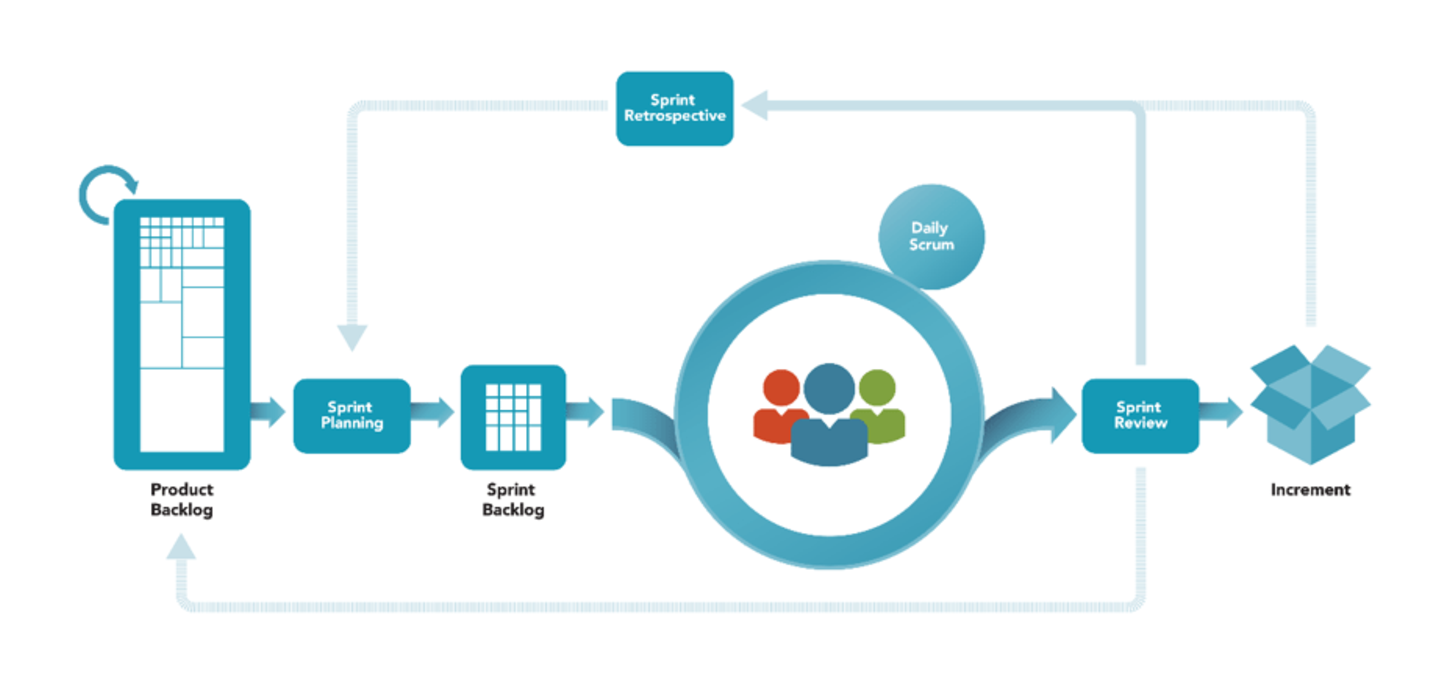
\includegraphics[width=1\textwidth]{figures/scrum}
		\caption{Proceso de desenvolvemento en Scrum.}
		\label{fig:scrum}
	\end{center}
\end{figure}

\subsection{Inicio de ciclo}

O ciclo iníciase coa xuntanza dos usuarios e clientes na que se describirán as súas necesidades e aportarán suxerencias. Posteriormente, o Product owner será o encargado de crear a lista coas tarefas ordenadas por prioridade en base a esas necesidades e suxerencias dos usuarios e clientes. Esa lista é o Product backlog.

\subsection{Sprint planning meeting}

Iníciase coa xuntanza para a planificación do sprint. O Scrum master estima, coa axuda do equipo Scrum, as tarefas incluídas no Product backlog e decídense cales se levarán a cabo no sprint en base ás prioridades marcadas polo Product owner. Esta decisión tómana o Scrum master e o Product owner. Unha vez seleccionadas e priorizadas obtense o Sprint backlog, o conxunto de tarefas ordenadas para a iteración. Debe ser unha relación de tarefas realista, xa que o sprint backlog non pode ser modificado durante o sprint.
Nesta xuntanza elabórase un documento chamado Sprint goal, no que se expoñen os acordos aos que se chegaron para alcanzar a seguinte entrega.

\subsection{Daily standup}

Durante o sprint fanse unhas xuntanzas diarias cunha duración máxima de quince minutos nas que se expón o estado do proxecto. Estas xuntanzas deben realizarse sempre á mesma hora e no mesmo lugar. Cada membro do equipo deber responder tres preguntan que axudan a dar unha visión do estado do proxecto:

\begin{itemize}
	\item Que fixeches dende a última Daily standup?
	\item Que tes pensado facer ata a próxima Daily standup?
	\item Houbo algún problema que che impedise alcanzar o teu obxectivo?
\end{itemize}

\subsection{Sprint review meeting}

Ao rematar o sprint hai que levar a cabo unha xuntanza para a súa revisión, na que se identifica o traballo completado e o que quedou inconcluso. Nesta xuntanza tamén se fai unha demostración do produto desenvolvido ao Product owner e ao cliente. Todas aquelas tarefas que se ensinen deben estar rematadas, non se mostra o produto a medias.

\subsection{Sprint retrospective}

Esta xuntanza tamén se realiza ao finalizar os sprints. O equipo ao completo avalía o que se fixo ben e o que se fixo mal para poder aprender dos erros e repetir os éxitos. Todos os membros do equipo teñen a posibilidade de comentar a súa opinión sobre o sprint co obxectivo de procurar unha mellora no proceso.

\section{Vantaxes e desvantaxes de Scrum}

\subsection{Vantaxes}

\begin{itemize}
	\item Os riscos son rapidamente identificados debido ás xuntanzas diarias, polo que poden ser tratados antes de que produzan problemas.
	\item Axeitado para desenvolvementos con moitos riscos xa que poden ser rapidamente codificados e probados.
	\item O avance no desenvolvemento do proxecto é claro debido ás xuntanzas diarias.
	\item O cliente pode revisar produtos frecuentemente, o que permite adaptarse a cambios suxeridos por el máis rapidamente debido ao seu feedback.
	\item As xuntanzas diarias permite medir a produtividade individual. Isto axuda á mellora na produtividade de cada un dos membros do equipo.
	\item Evita o custo asociado á xestión do proceso, o que provoca un proxecto máis barato.
\end{itemize}

\subsection{Desvantaxes}

\begin{itemize}
	\item Require a plena disposición dos membros do equipo.
	\item Non se axusta demasiado ben a proxectos grandes con varios equipos traballando en conxunto.
	\item Esta metodoloxía require de membros con experiencia, xa que a planificación non depende do traballador que realice a tarefa. Tamén se debe a que todos os membros deben realizar análises, deseños, implementacións e probas.
	\item Se algunha das tarefas non está ben definida, o tempo e os custos do sprint non será realista. Este problema pode prolongarse durante varios sprints.
	\item Se a xerencia non confía completamente nos membros do equipo esta metodoloxía non é axeitada pois dá moita liberdade.
	\item Se non se ten unha data de fin do proxecto clara e definida o cliente pode seguir demandando novas tarefas sen límite.
\end{itemize}


\section{Adaptación da metodoloxía}
Aínda que se teñan claras todas as vantaxes propias desta metodoloxía, non se pode aplicar ao pé da letra pois o equipo de desenvolvemento consta dunha única persoa. Debido a isto, débese adaptar a metodoloxía ao noso caso. Por unha parte optouse por non levar a cabo as xuntanzas diarias e pola outra, que as reunións co titor funcionasen como as xuntanzas de inicio e fin de sprint, coincidindo no tempo. A duración dos sprints non serán fixas durante o proxecto, senón que estarán comprendida entre os 15 e os 20 días, aproximadamente.
Os roles estarán repartidos entre o alumno, que será tanto o equipo de desenvolvemento coma o scrum master no día a día; e o titor, que se encargará de adoptar a figura de scrum master nas xuntanzas entre sprints.
